\documentclass{beamer}
\setbeamertemplate{caption}[numbered]
\usepackage{graphicx}
\usepackage[utf8]{inputenc}
\usepackage[english]{babel}
\graphicspath{{Images/}}
\usepackage{comment}
\usepackage{verbatim}
\usepackage{hyperref}
\mode<presentation>
{
	\usetheme{AnnArbor}
	\usecolortheme{crane}
}

\title{ISRC Workshop}
\subtitle[Intro to Stata]{Introduction to Stata}
\author[Wallace]{Desmond D. Wallace}
\institute[University of Iowa]{Department of Political Science\\The University of Iowa\\Iowa City, IA}

\date{September 15, 2017}

\begin{document}
	
\begin{frame}
	\titlepage
\end{frame}

\section{Stata Interface}
\subsection{Main Window}

\begin{frame}
	\frametitle{PC}
		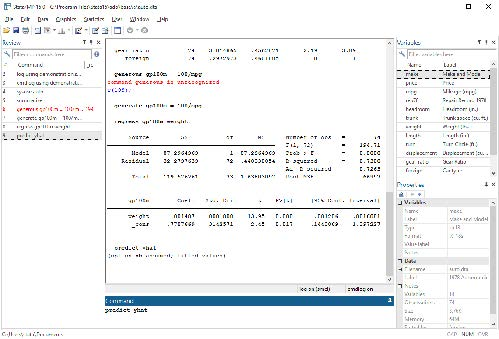
\includegraphics[scale=0.75]{main_window_pc}
\end{frame}

\begin{frame}
	\frametitle{MAC}
		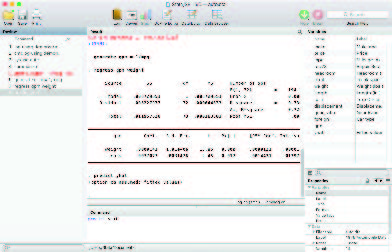
\includegraphics[scale=0.75]{main_window_mac}
\end{frame}

\begin{frame}
	\frametitle{Descriptions}
		\begin{enumerate}
			\item Command -- Type commands
			\item Results -- Executed commands and resulting output
			\begin{enumerate}
				\item Current and Command log status
			\end{enumerate}
			\item Review -- Past commands from current session
			\item Variables -- Variable list of current dataset
			\item Properties -- Displays dataset and variable properties
		\end{enumerate}
		Note: Grey Bar at Bottom of the Screen -- Displays current working directory
\end{frame}

\subsection{Toolbar}

\begin{frame}
	\frametitle{PC and MAC}
		PC: 
\includegraphics[scale=0.75]{toolbar_pc} \\
		MAC: 
\includegraphics[scale=0.25]{toolbar_mac}
\end{frame}

\begin{frame}
	\frametitle{Descriptions}
		\begin{itemize}
			\item Open -- Open a Stata-related file
			\item Save -- Save a Stata-related file
			\item Print -- Print output displayed in the results window
			\item Log -- Begin, close, suspend, or resume a log file
			\item Viewer -- Displays help files
			\item Graph -- Launches the graph window
		\end{itemize}
\end{frame}

\begin{frame}
	\frametitle{Descriptions}
		\begin{itemize}
			\item Do-file Editor -- Launches the Do-file editor
			\item Data Editor/Browser -- Launches the Data viewer
			\item Variables Manager -- Lists the variables in the current dataset; allows for the editing of variables
			\item More -- Display results that do not fit in the results window
			\item Break -- Stops the execution of a command
			\item Search Help -- Searches for help for Stata-written and user-written commands
		\end{itemize}
\end{frame}

\subsection{Data Browser}

\begin{frame}
	\frametitle{PC}
		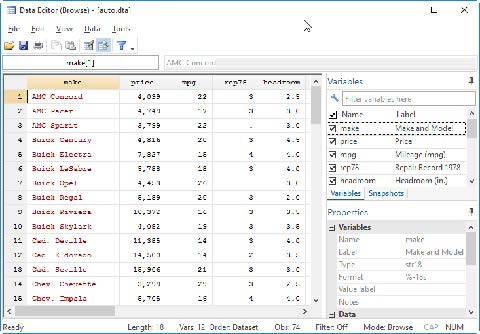
\includegraphics[scale=0.75]{data_editor_pc}
\end{frame}

\begin{frame}
	\frametitle{MAC}
		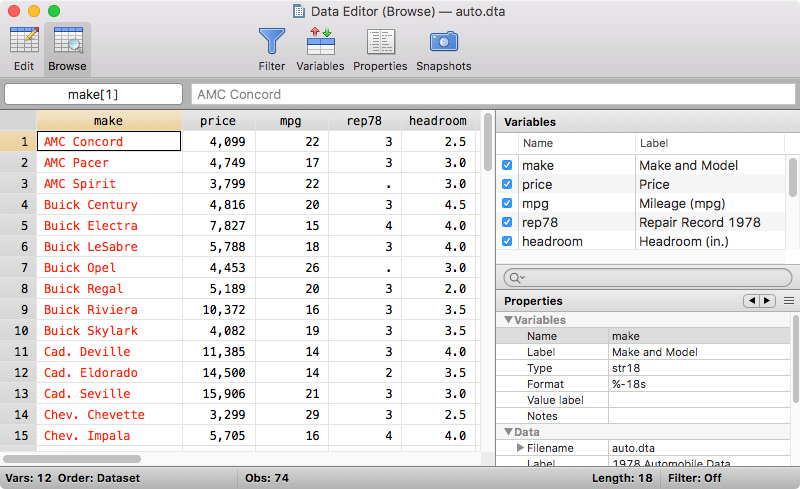
\includegraphics[scale=0.35]{data_editor_mac}
\end{frame}

\begin{frame}
	\frametitle{Modes}
		\begin{itemize}
			\item Data Editor (Edit) -- Allows one to view a dataset, and make changes
			\item Data Editor (Browse) -- Allows one to view the dataset, but not make any changes
			\item Can switch between edit mode and browse mode
			\item NOTE: When switching from browse mode to edit mode, a warning will appear, whether the user is sure about switching from browse mode to edit mode
		\end{itemize}
\end{frame}

\begin{frame}
	\frametitle{Colors}
		When viewing a dataset in the Data Editor/Browser, different types of data is represented by different colors
		\begin{itemize}
			\item Black -- Data used for various descriptive and analytic tasks
			\item Red -- Observations that contain strings, or textual data; can perform descriptive tasks, but not analytic tasks
			\item Blue -- Same as data appearing in black, except the blue represents value labels; can perform both descriptive and analytic tasks
			\item NOTE: Default is for the Data Editor/Browser to display the value labels, if any for the variables
		\end{itemize}
\end{frame}

\section{Stata Commands}
\subsection{General Command Syntax}

\begin{frame}
	\frametitle{Full Command Syntax}
		{\tiny [\textbf{by} \textit{varlist}:] \textit{command} [\textit{varlist}] [=\textit{exp}] [\textbf{if} \textit{exp}] [\textbf{in} \textit{range}] [\textit{weight}] [\textbf{using} \textit{filename}] [,\textit{options}]}
\end{frame}

\subsection{Descriptions}

\begin{frame}
	\frametitle{\textit{command}}
		\begin{itemize}
			\item Only required element of command statement
			\item Case-sensitive
			\item Commands can be abbreviated
			\item Example: To display summary statistics of a variable, or variables:
			\begin{itemize}
				\item \texttt{\underline{sum}merize}
				\item \texttt{sum}
				\item The underlined portion of \texttt{summerize} represents the abbreviation
			\end{itemize}
		\end{itemize}
\end{frame}

\begin{frame}
	\frametitle{\textit{varlist}}
		\begin{itemize}
			\item Represents one variable, or at least two variables
			\item Case-sensitive
			\item Variables can be abbreviated to minimum number of letters that makes variable unique
			\item To refer to several variables at the same time:
				\begin{itemize}
					\item Use the * symbol
					\item Use a name range
				\end{itemize}
		\end{itemize}
\end{frame}

\begin{frame}
	\frametitle{\textit{=exp}}
		\begin{itemize}
			\item Used to generate new variables
			\item Can include variables in expression statements
			\item Usually an arithmetic expression
				\begin{itemize}
					\item Can include the four basic operation symbols ($+$, $-$, $*$, $/$)
					\item Can use \^{} for an exponentiation statement
					\item Can include other functions, such as $abs$ and $log$
					\item Can include parentheses to manage order of operations
				\end{itemize}
		\end{itemize}
\end{frame}

\begin{frame}
	\frametitle{if \textit{exp} and in \textit{range}}
		\begin{itemize}
			\item Used to restrict dataset to a subsample of interest
			\item Represented as a logical statement that is either true or false
			\item Relation operators are $<$, $<=$, $==$, $>=$, $>$, and $!=$
			\item Can also specify a range of observations
			\item Example: \texttt{in 1/10} refers to the first ten observations of a dataset
		\end{itemize}
\end{frame}

\begin{frame}
	\frametitle{\textit{weights}}
		\begin{itemize}
			\item Used to weigh the observations
			\item Example: survey data typically uses weights in order to make the sample representative of the population
			\item Used in conjunction with many commands
		\end{itemize}
\end{frame}

\begin{frame}
	\frametitle{using \textit{filename}}
		\begin{itemize}
			\item Introduces a file into the command
			\item File can be on the computer, on a network, or on the internet
		\end{itemize}
\end{frame}

\begin{frame}
	\frametitle{\textit{options}}
		\begin{itemize}
			\item Most commands have additional options that the user can specify
			\item Look at the help file for the command to list its options
		\end{itemize}
\end{frame}

\begin{frame}
	\frametitle{by \textit{varlist}}
		\begin{itemize}
			\item Used to execute a command for groups of observations defined by distinct values of the variable(s) specified
			\item Command in question has to be "byable"
			\item Data must be sorted by the grouping variable
			\item If data is not pre-sorted, use \texttt{bysort}
		\end{itemize}
\end{frame}

\subsection{Hypothesis}

\begin{frame}
	\frametitle{Interdependent Responsiveness}
		\textit{\underline{Interdependent Responsiveness Hypothesis}: The effect public opinion has on policy output, in the presence of interdependence, is different compared to not accounting for interdependence.}
\end{frame}

\section{Research Design}
\subsection{Methodology}

\begin{frame}
	\frametitle{m-STAR Model}
		\[y=Wy+\phi My+X\beta+\epsilon\]
		\[W\equiv\sum^{R}_{r=1}\rho_{r}W_{r}\]
\end{frame}

\subsection{Data}

\begin{frame}
	\frametitle{Dependent Variables}
		\[\alert{y}=Wy+\phi My+X\beta+\epsilon\]
		\begin{enumerate}
			\item Policy Priority Scores (Jacoby and Schneider (2009))
			\item \alert{Policy Liberalism Scores (Caughey and Warshaw (2016))}
		\end{enumerate}
\end{frame}

\begin{frame}
	\frametitle{Spatial Lag Variables}
		\[y=\alert{Wy}+\phi My+X\beta+\epsilon\]
		\[W=\rho_{1}W_{1}+\rho_{2}W_{2}+\rho_{3}W_{3}\]
		\begin{enumerate}
			\item Learning -- Geographic Contiguity (Dichotomous)
			\item Imitation -- Government Partisan Composition (Dichotomous)
			\item Competition -- Gross State Product per Capita (Absolute difference)
		\end{enumerate}
\end{frame}

\begin{frame}
	\frametitle{Independent Variable and Controls}
		\[y=Wy+\phi My+\alert{X\beta}+\epsilon\]
		\begin{enumerate}
			\item Citizen Policy Liberalism (Caughey and Warshaw (2015))
			\item Controls
			\begin{enumerate}
				\item Political (Govt. Ideology, self-ID Liberals and Democrats)
				\item Socioeconomic (Disposable personal income, minority population percentage, educational attainment)
				\item Temporal Quadratic Polynomial Function (Time, $\mbox{Time}^2$)
			\end{enumerate}
		\end{enumerate}
\end{frame}

\section{Results}
\subsection{Model}

\begin{frame}
	\frametitle{Model Results}
	{\scriptsize\begin{table}[]
			\centering
			\caption{DV -- Policy Liberalism Score}
			\label{tab:tab1}
			\begin{tabular}{cccccc}
				& (1)                                                            & (2)                                                            & (3)                                                             & (4)                                                             & (5)                                                            \\
				& b/se                                                           & b/se                                                           & b/se                                                            & b/se                                                            & b/se                                                           \\
				Geographic Contiguity      & \begin{tabular}[c]{@{}l@{}}0.553***\\ (0.027)\end{tabular} &                                                                &                                                                 & \begin{tabular}[c]{@{}l@{}}0.057\\ (0.063)\end{tabular}     &                                                                \\
				Govt. Partisan Composition       &                                                                & \begin{tabular}[c]{@{}l@{}}-0.005\\ (0.057)\end{tabular}   &                                                                 & \begin{tabular}[c]{@{}l@{}}0.501***\\ (0.026)\end{tabular}  &                                                                \\
				GSP per capita    &                                                                &                                                                & \begin{tabular}[c]{@{}l@{}}-2.986***\\ (0.394)\end{tabular} & \begin{tabular}[c]{@{}l@{}}-3.028***\\ (0.358)\end{tabular} &                                                                \\
				Citizen Policy Liberalism & \begin{tabular}[c]{@{}l@{}}0.380***\\ (0.138)\end{tabular} & \begin{tabular}[c]{@{}l@{}}0.904***\\ (0.155)\end{tabular} & \begin{tabular}[c]{@{}l@{}}0.782***\\ (0.147)\end{tabular}  & \begin{tabular}[c]{@{}l@{}}0.381***\\ (0.133)\end{tabular}  & \begin{tabular}[c]{@{}l@{}}0.904***\\ (0.155)\end{tabular}
			\end{tabular}
	\end{table}}
\end{frame}

\subsection{Interpretation}

\begin{frame}
	\frametitle{Average Direct, Indirect, and Total Effects}
	{\normalsize\begin{table}[]
			\centering
			\caption{DV -- Policy Liberalism Score}
			\label{tab:tab2}
			\begin{tabular}{@{}llccl@{}}
				&                                       & \multicolumn{2}{c}{\textbf{Model Type}}     &  \\
				&                                       & \textit{Spatial}     & \textit{Non-spatial} &  \\
				& \multicolumn{1}{c}{\textit{Avg. Direct}}   & 0.400             & 0.904             &  \\
				\multicolumn{1}{c}{\textbf{\begin{tabular}[c]{@{}c@{}}Effects\\ Type\end{tabular}}} & \multicolumn{1}{c}{\textit{Avg. Indirect}} & -0.294             & 0                    &  \\
				& \multicolumn{1}{c}{\textit{Avg. Total}}    & 0.107             & 0.904             &  \\
			\end{tabular}
	\end{table}}
	{\footnotesize\begin{itemize}
			\item Avg. Direct: Average of main diagonal elements of marginal change matrix.
			\item Avg. Indirect: Average of off-diagonal elements of marginal change matrix.
			\item Avg. Total: Average of all elements of marginal change matrix.
	\end{itemize}}
\end{frame}

\section{Conclusions}

\begin{frame}
	\frametitle{Summarized Results}
	\begin{itemize}
		\item States' response to citizen policy liberalism shocks in another state is to make opposite policy decisions.
		\item Interdependence has a negative effect on policy responsiveness.
		\item Implication: Need to account for interdependence when studying responsiveness and representation.
	\end{itemize}
\end{frame}

\begin{frame}
	\begin{center}
		\begin{LARGE}
			Any Questions?
		\end{LARGE}
	\end{center}
\end{frame}

\end{document}
